% Figure: the diffusion adapter oracle pipeline.
% Compile: latexmk -pdf fig_architecture.tex   (standalone class; \includegraphics the PDF)
% Style: one node style per kind of thing, explicit positioning offsets in consistent multiples,
% arrows between named node borders only, thin lines, fill encodes exactly one category
% (shaded = frozen, white = trained); the caption states the encoding.
\documentclass[tikz,border=2pt]{standalone}
\usetikzlibrary{positioning,arrows.meta}
\begin{document}
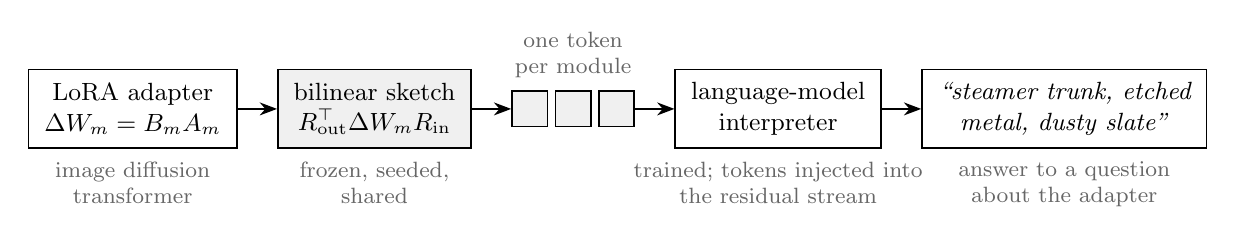
\begin{tikzpicture}[
  font=\small,
  every node/.style={align=center},
  tensor/.style ={draw, line width=0.6pt, minimum height=10mm, inner xsep=2mm, fill=white},
  frozen/.style ={draw, line width=0.6pt, minimum height=10mm, inner xsep=2mm, fill=black!6},
  trained/.style={draw, line width=0.6pt, minimum height=10mm, inner xsep=2mm, fill=white},
  txt/.style    ={draw, line width=0.6pt, minimum height=10mm, inner xsep=2mm, fill=white,
                  font=\small\itshape},
  tok/.style    ={draw, line width=0.6pt, minimum size=4.5mm, inner sep=0pt, fill=black!6},
  flow/.style   ={-{Stealth[length=2.2mm]}, line width=0.6pt},
  lbl/.style    ={font=\footnotesize, text=black!60, inner sep=1.5pt},
]

\node[tensor] (adapter) at (0,0) {LoRA adapter\\ $\Delta W_m = B_m A_m$};
\node[lbl, below=1mm of adapter] {image diffusion\\ transformer};

\node[frozen, right=5mm of adapter] (encoder)
  {bilinear sketch\\ $R_{\mathrm{out}}^\top \Delta W_m R_{\mathrm{in}}$};
\node[lbl, below=1mm of encoder] {frozen, seeded,\\ shared};

\node[tok, right=5mm of encoder] (t1) {};
\node[tok, right=0.8mm of t1]    (t2) {};
\node[tok, right=0.8mm of t2]    (t3) {};
\node[lbl, above=1mm of t2] {one token\\ per module};

\node[trained, right=5mm of t3] (reader)
  {language-model\\ interpreter};
\node[lbl, below=1mm of reader] {trained; tokens injected into\\ the residual stream};

\node[txt, right=5mm of reader] (answer)
  {``steamer trunk, etched\\ metal, dusty slate''};
\node[lbl, below=1mm of answer] {answer to a question\\ about the adapter};

\draw[flow] (adapter) -- (encoder);
\draw[flow] (encoder) -- (t1);
\draw[flow] (t3) -- (reader);
\draw[flow] (reader) -- (answer);

\end{tikzpicture}
\end{document}
